% ------------------------------------------------------------------------------
% TYPO3 v9 LTS - What's New (English Version)
%
% @author	Michael Schams <schams.net>
% @license	Creative Commons BY-NC-SA 3.0
% @link		https://typo3.org/help/documentation/whats-new/
% @language	English
% ------------------------------------------------------------------------------

\section{In-depth Changes}
\begin{frame}[fragile]
	\frametitle{In-depth Changes}

	\begin{center}\huge{\color{typo3darkgrey}\textbf{In-depth Changes}}\end{center}
	\begin{center}\large{\textit{Candy for Integrators and Developers}}\end{center}

\end{frame}

% Candy for Integrators and Developers
% Awesome new features and improvements under the hood

% ------------------------------------------------------------------------------
% Management Database Columns
% #85160 - Auto create management DB fields from TCA ctrl

\begin{frame}[fragile]
	\frametitle{In-depth Changes}
	\framesubtitle{"Management" Database Columns}

	\begin{itemize}
		\item Database schema analyzer automatically creates TYPO3 "management"
			columns by reading the TCA
		\item Developers do not need to state these fields in file
			\texttt{ext\_tables.sql}
		\item Management fields are for example:\newline
			\texttt{uid}, \texttt{pid}, \texttt{crdate}, \texttt{cruser},
			\texttt{hidden}, \texttt{deleted}, \texttt{sortby}, etc.\newline
			\small(also fields used for translations, versioning, workspaces)\normalsize
		\item Field definitions in \texttt{ext\_tables.sql} take precedence
			over automatically generated fields, which means they can be
			customized if required
		\item See \href{https://docs.typo3.org/typo3cms/extensions/core/latest/Changelog/9.3/Feature-85160-AutoCreateManagementDBFieldsFromTCACtrl.html}{documentation}
			for further details
	\end{itemize}

\end{frame}

% ------------------------------------------------------------------------------
% #85389 - Introduce Context API for consistent data handling

\begin{frame}[fragile]
	\frametitle{In-depth Changes}
	\framesubtitle{Context API}

	\begin{itemize}
		\item A new Context API was introduced in TYPO3 version 9.4
		\item The main goal of this concept is to centralize global variables
		\item The API aims to replace globally available objects (e.g.
			\texttt{TSFE}, \texttt{sys\_page}, \texttt{BE\_USER}, etc.) and to
			make them available in a common, structured and logical way
		\item Instead of exposing a full object (e.g. the \texttt{BE\_USER}
			object), "aspects" contain properties, which are relevant and
			required only
		\item Extension developers can add aspects to the current context
		\item See \href{https://docs.typo3.org/typo3cms/extensions/core/latest/Changelog/9.4/Feature-85389-ContextAPIForConsistentDataHandling.html}{documentation}
			for further details and examples how to use the API
	\end{itemize}

\end{frame}

% ------------------------------------------------------------------------------
% Feature Toggles

\begin{frame}[fragile]
	\frametitle{In-depth Changes}
	\framesubtitle{Feature Toggles}

	\begin{itemize}
		\item You can now enable or disable core feature with a new function:
			\href{https://docs.typo3.org/typo3cms/CoreApiReference/ApiOverview/FeatureToggles/}{Feature Toggle}
			(under ADMIN TOOLS → Settings)
	\end{itemize}

	\begin{figure}
		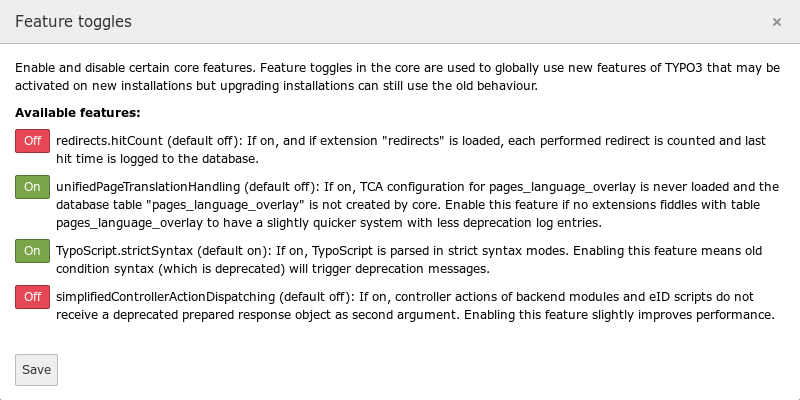
\includegraphics[width=0.70\linewidth]{InDepthChanges/FeatureToggles.png}
	\end{figure}

\end{frame}

% ------------------------------------------------------------------------------
% Feature Toggles

\begin{frame}[fragile]
	\frametitle{In-depth Changes}
	\framesubtitle{Feature Toggles}

	\begin{itemize}
		\item The Feature Toggle lets developers implement features in parallel
			to their legacy version
		\item Integrators and site administrators can decide when they want to
			switch to new features
		\item Developers can leverage an API class
		\item This also means that the TYPO3 core and extensions can provide
			alternative functionality for a certain feature
	\end{itemize}

\end{frame}

% ------------------------------------------------------------------------------
% #85829 - Implement symfony expression language for TypoScript conditions
% #86068 - Deprecate old condition syntax

\begin{frame}[fragile]
	\frametitle{In-depth Changes}
	\framesubtitle{Symfony ExpressionLanguage}

	% decrease font size for code listing
	\lstset{basicstyle=\tiny\ttfamily}

	\begin{itemize}
		\item The \href{https://symfony.com/doc/current/components/expression_language/syntax.html}{Symfony ExpressionLanguage}
			component has been implemented for TypoScript conditions (frontend
			and backend)
		\item Some examples:

\begin{lstlisting}
[page["uid"] in 18..45]
# This condition matches, if current page uid is between 18 and 45
[END]

[not ("foo" matches "/bar/")]
# This condition matches, if "foo" does not match the regular expression '/bar/'
[END]

[request.getNormalizedParams().getHttpHost() == 'example.com']
# This condition matches, if current hostname is 'example.com'
[END]
\end{lstlisting}

		\item Using old condition syntax triggers a deprecation message
	\end{itemize}

\end{frame}

% ------------------------------------------------------------------------------
% #85828 - Move symfony expression language handling into EXT:core

\begin{frame}[fragile]
	\frametitle{In-depth Changes}
	\framesubtitle{Symfony ExpressionLanguage}

	% decrease font size for code listing
	\lstset{basicstyle=\tiny\ttfamily}

	\begin{itemize}
		\item Expression Language can also be used in your custom code
		\item The TYPO3 core features the class \texttt{DefaultProvider}, which
			can be used directly (see example below) and custom implementations
			can extend the class \texttt{AbstractProvider}

\begin{lstlisting}
use \TYPO3\CMS\Core\ExpressionLanguage\DefaultProvider;
use \TYPO3\CMS\Core\ExpressionLanguage\Resolver;

$provider = GeneralUtility::makeInstance(DefaultProvider::class);
$conditionResolver = GeneralUtility::makeInstance(Resolver::class, $provider);
$conditionResolver->evaluate('1 < 2'); // result is true
\end{lstlisting}

	\end{itemize}

\end{frame}

% ------------------------------------------------------------------------------
% #85256 - Install TYPO3 on SQLite

\begin{frame}[fragile]
	\frametitle{In-depth Changes}
	\framesubtitle{Install TYPO3 on SQLite}

	\begin{itemize}
		\item TYPO3 now supports \href{https://www.sqlite.org}{SQLite},
			a self-contained, lightweight open source SQL database engine
		\item SQLite can be selected during the web-based installation process,
			if PHP module "pdo\_sqlite" is installed and enabled:
	\end{itemize}

	\begin{figure}
		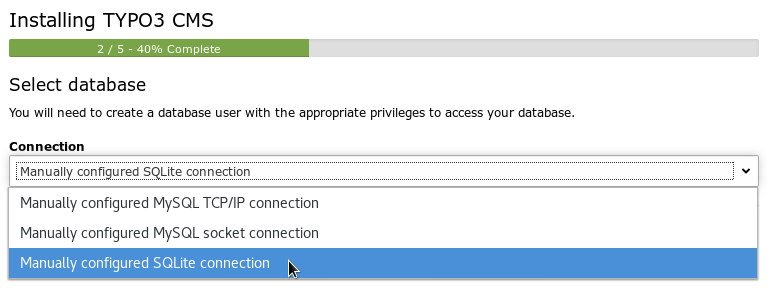
\includegraphics[width=0.65\linewidth]{InDepthChanges/85256-InstallTYPO3OnSQLite.png}
	\end{figure}

\end{frame}
% ------------------------------------------------------------------------------
% #85256 - Install TYPO3 on SQLite

\begin{frame}[fragile]
	\frametitle{In-depth Changes}
	\framesubtitle{Install TYPO3 on SQLite}

	\begin{itemize}
		\item Database is stored in a single file, which means TYPO3 instances
			can now run natively in PHP, including the data storage
		\item Using SQLite makes sense for relatively small TYPO3 sites
			or e.g. for test and development instances
		\item System administrators should take appropriate actions to protect
			the \texttt{*.sqlite} file from unauthorized access if the file
			is stored inside the web container (depends on type of setup)
	\end{itemize}

\end{frame}

% ------------------------------------------------------------------------------
% #83461 - Show Fieldname Next To Title In Debug Mode

\begin{frame}[fragile]
	\frametitle{In-depth Changes}
	\framesubtitle{Field Names in Debug Mode}

	\begin{itemize}

		\item TYPO3 integrators and developers often deal with input fields in the backend,
			e.g. when setting up access permissions or during TsConfig configuration

		\item Instead of having to look into the source code of the browser,
			field names are now displayed for each field generated by the
			FormEngine now

		\item This only applies to users with administrator privileges and
			requires that the debug mode is enabled in TYPO3:

			\smaller
				\texttt{\$GLOBALS['TYPO3\_CONF\_VARS']['BE']['debug']}
			\normalsize

	\end{itemize}

	\begin{figure}
		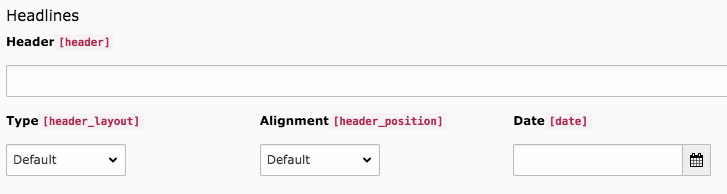
\includegraphics[width=0.60\linewidth]{InDepthChanges/83461-ShowFieldnameNextToTitleInDebugMode.png}
	\end{figure}

\end{frame}

% ------------------------------------------------------------------------------
% Mail Queue (SwiftMailer)

\begin{frame}[fragile]
	\frametitle{In-depth Changes}
	\framesubtitle{Mail Queue}

	% decrease font size for code listing
	\lstset{basicstyle=\tiny\ttfamily}

	\begin{itemize}
		\item Emails generated by TYPO3 are sent out immediately by default
		\item TYPO3 v9 LTS now supports
			\href{https://swiftmailer.symfony.com/}{SwiftMailer's} spool functionality,
			where message are saved in a queue first and processed later

		\item Option 1: spool mails in memory\newline
			\smaller
				(emails are only sent, if request got executed without any exceptions or errors)
			\normalsize

\begin{lstlisting}
$GLOBALS['TYPO3_CONF_VARS']['MAIL']['transport_spool_type'] = 'memory';
\end{lstlisting}

		\item Option 2: spool mails in files

\begin{lstlisting}
$GLOBALS['TYPO3_CONF_VARS']['MAIL']['transport_spool_type'] = 'file';
$GLOBALS['TYPO3_CONF_VARS']['MAIL']['transport_spool_filepath'] = '/folder/of/choice';
\end{lstlisting}

	\end{itemize}

\end{frame}

% ------------------------------------------------------------------------------
% Mail Queue (SwiftMailer)

\begin{frame}[fragile]
	\frametitle{In-depth Changes}
	\framesubtitle{Mail Queue}

	% decrease font size for code listing
	\lstset{basicstyle=\tiny\ttfamily}

	\begin{itemize}
		\item The following console command can be used to process the queue and send
			out spooled emails
			\newline\newline
			\small
				Process all spooled emails:
			\normalsize
\begin{lstlisting}
$ ./typo3/sysext/core/bin/typo3 swiftmailer:spool:send
\end{lstlisting}

			\small
				Process spooled emails, but not more than 10 messages:
			\normalsize
\begin{lstlisting}
$ ./typo3/sysext/core/bin/typo3 swiftmailer:spool:send --message-limit=10
\end{lstlisting}

			\small
				Process spooled emails, but no longer than 10 seconds:
			\normalsize
\begin{lstlisting}
$ ./typo3/sysext/core/bin/typo3 swiftmailer:spool:send --time-limit=10
\end{lstlisting}

	\end{itemize}

\end{frame}

% ------------------------------------------------------------------------------
% Extension Scanner

\begin{frame}[fragile]
	\frametitle{In-depth Changes}
	\framesubtitle{Extension Scanner}

	\begin{itemize}
		\item An Extension Scanner has been added to TYPO3 that aims to help
			when upgrading TYPO3 from one major version to the next
		\item This tool can scan extension code for the usage of TYPO3 core
			APIs which have been removed or marked deprecated
		\item The result is a detailed overview of actions required
		\item If available, it references to appropriate documentation on how to
			migrate the code in question
		\item Standalone tool \href{https://github.com/Tuurlijk/typo3scan}{TYPO3 Scanner}
			(by Michiel Roos)
		\item Further details in a \href{https://www.youtube.com/watch?v=UdIYDZgBrQU}{video on YouTube}
			(by TYPO3 GmbH)
	\end{itemize}

\end{frame}

% ------------------------------------------------------------------------------
% Extension Scanner

\begin{frame}[fragile]
	\frametitle{In-depth Changes}
	\framesubtitle{Extension Scanner (in TYPO3 v9 LTS)}

	\begin{figure}
		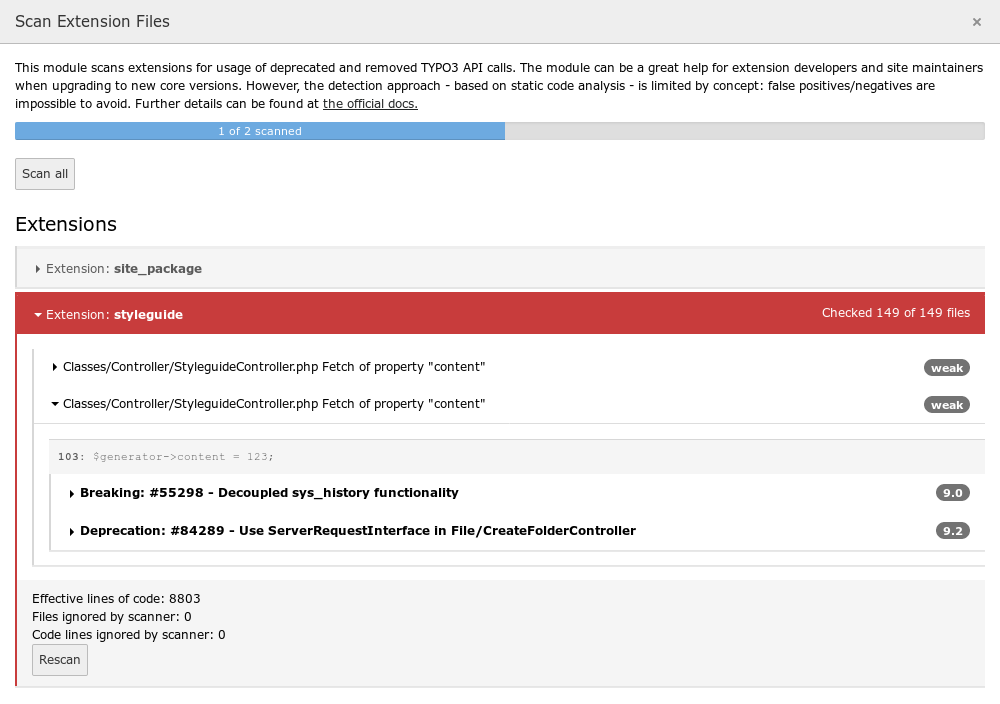
\includegraphics[width=0.70\linewidth]{InDepthChanges/ExtensionScanner.png}
	\end{figure}

\end{frame}

% ------------------------------------------------------------------------------
% Extension Scanner

\begin{frame}[fragile]
	\frametitle{In-depth Changes}
	\framesubtitle{Extension Scanner (Standalone)}

	\begin{figure}
		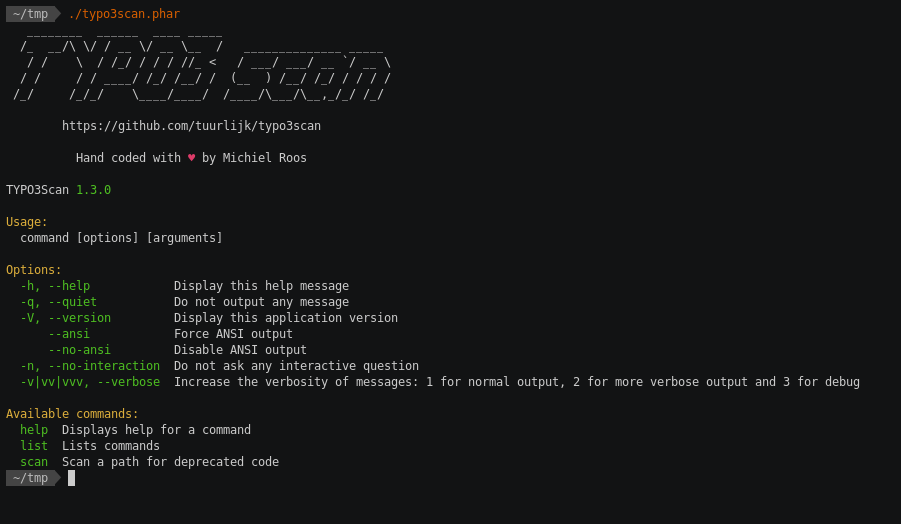
\includegraphics[width=0.70\linewidth]{InDepthChanges/Typo3Scanner.png}
	\end{figure}

\end{frame}

% ------------------------------------------------------------------------------
% #82363 - Make Extbase translation handling consistent with TypoScript

\begin{frame}[fragile]
	\frametitle{In-depth Changes}
	\framesubtitle{Extbase Translation Handling}

	% decrease font size for code listing
	\lstset{basicstyle=\footnotesize\ttfamily}

	\begin{itemize}
		\item Extbase now renders translated records the same way as TypoScript
			does
		\item The new behaviour is controlled by the feature switch:

\begin{lstlisting}
config.tx_extbase.features.consistentTranslationOverlayHandling
  = 1
\end{lstlisting}

		\item The new behaviour is the default in v9 LTS (the feature switch
			will be removed in v10)
		\item Learn more about how to query data using Extbase in the
			\href{https://docs.typo3.org/typo3cms/extensions/core/latest/Changelog/9.5/Important-82363-MakeExtBaseTranslationHandlingConsistentWithTyposcript.html}{TYPO3 documentation}

	\end{itemize}

\end{frame}

% ------------------------------------------------------------------------------
% PSR-3, PSR-7 and PSR-15

\begin{frame}[fragile]
	\frametitle{In-depth Changes}
	\framesubtitle{PHP Standard Recommendation (PSR)}

	\begin{itemize}
		\item The
			\href{https://www.php-fig.org/psr/}{PHP Standard Recommendation (PSR)}
			is a specification published by the PHP Framework Interop Group
		\item TYPO3 introduced PSR-15 middleware in the frontend and backend
		\item All web requests in the TYPO3 core return a response that complies
			with PSR-7, the standard for HTTP message interfaces
		\item The PSR-3 standard describes a logging interface for PHP
			applications, which is used by all logging procedures throughout
			the TYPO3 system now
	\end{itemize}

\end{frame}

% ------------------------------------------------------------------------------
